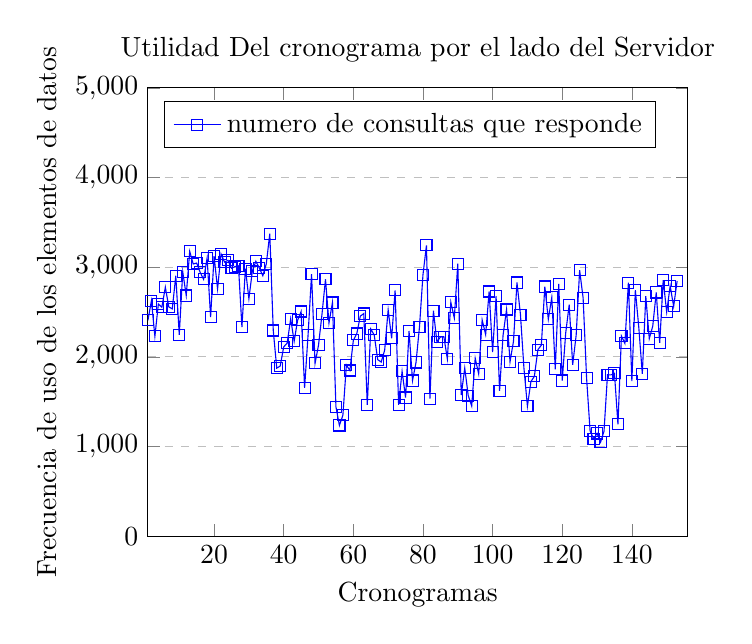
\begin{tikzpicture}
\begin{axis}[
    title={Utilidad Del cronograma por el lado del Servidor},
    xlabel={Cronogramas},
    ylabel={Frecuencia de uso de los elementos de datos},
    xmin=1, xmax=156,
    ymin=0, ymax=5000,
    xtick={},
    ytick={},
    legend pos=north west,
    ymajorgrids=true,
    grid style=dashed,
]

\addplot[
    color=blue,
    mark=square,
    ]
    coordinates {
%UTILIDAD TOTAL
(1,2407)
(2,2626)
(3,2229)
(4,2590)
(5,2553)
(6,2777)
(7,2556)
(8,2536)
(9,2904)
(10,2246)
(11,2948)
(12,2684)
(13,3177)
(14,3036)
(15,3046)
(16,2943)
(17,2865)
(18,3102)
(19,2444)
(20,3124)
(21,2758)
(22,3148)
(23,3057)
(24,3077)
(25,2988)
(26,3007)
(27,3015)
(28,2333)
(29,2983)
(30,2649)
(31,2958)
(32,3066)
(33,2990)
(34,2905)
(35,3037)
(36,3374)
(37,2294)
(38,1874)
(39,1898)
(40,2111)
(41,2154)
(42,2425)
(43,2174)
(44,2409)
(45,2506)
(46,1654)
(47,2247)
(48,2922)
(49,1927)
(50,2131)
(51,2477)
(52,2865)
(53,2378)
(54,2606)
(55,1443)
(56,1235)
(57,1350)
(58,1909)
(59,1848)
(60,2184)
(61,2260)
(62,2454)
(63,2483)
(64,1465)
(65,2311)
(66,2243)
(67,1969)
(68,1942)
(69,2075)
(70,2524)
(71,2207)
(72,2742)
(73,1465)
(74,1838)
(75,1546)
(76,2288)
(77,1736)
(78,1938)
(79,2335)
(80,2915)
(81,3244)
(82,1534)
(83,2514)
(84,2168)
(85,2221)
(86,2225)
(87,1977)
(88,2609)
(89,2433)
(90,3039)
(91,1575)
(92,1875)
(93,1567)
(94,1451)
(95,1984)
(96,1809)
(97,2412)
(98,2248)
(99,2729)
(100,2054)
(101,2676)
(102,1620)
(103,2240)
(104,2528)
(105,1944)
(106,2174)
(107,2829)
(108,2471)
(109,1874)
(110,1450)
(111,1724)
(112,1783)
(113,2080)
(114,2130)
(115,2784)
(116,2419)
(117,2663)
(118,1861)
(119,2814)
(120,1736)
(121,2268)
(122,2581)
(123,1911)
(124,2241)
(125,2966)
(126,2656)
(127,1760)
(128,1175)
(129,1085)
(130,1146)
(131,1048)
(132,1170)
(133,1800)
(134,1799)
(135,1817)
(136,1248)
(137,2232)
(138,2150)
(139,2828)
(140,1729)
(141,2745)
(142,2323)
(143,1811)
(144,2676)
(145,2203)
(146,2343)
(147,2718)
(148,2155)
(149,2856)
(150,2501)
(151,2791)
(152,2563)
(153,2846)
    };
    \legend{numero de consultas que responde}

\end{axis}
\end{tikzpicture}

